\documentclass{sosg-informe}

\graphicspath{{../../geodatos/estudios/santa-cruz/figuras/}{../../geodatos/estudios/san-cristobal/figuras/}{figuras/}}

\title{Modelo hidrodinámico 2D \enquote{rain-on-grid}\\del evento del 30 de octubre de 2026\\en Santa Cruz y San Cristóbal (Galápagos)}
\titulocorto{Modelo 2D rain-on-grid del 30-oct}
\numero{2026-06}
\estado{Borrador para discusión}
\titulocita{Modelo hidrodinámico 2D «rain-on-grid» del evento del 30 de octubre de 2026 en Santa Cruz y San Cristóbal (Galápagos)}
\relacionados{Issues \issue{13}, \issue{16}, \issue{26}, \issue{52} y \issue{74} · repositorio mayait/sosgalapagos-datos}
\date{4 de noviembre de 2026}

\begin{document}
\maketitle

\begin{abstract}
Se construyó un modelo hidrodinámico bidimensional \enquote{rain-on-grid} para reproducir la inundación del 30 de octubre de 2026 en La Cascada (Puerto Ayora, Santa Cruz) y explorar la respuesta de Puerto Baquerizo Moreno y El Progreso (San Cristóbal). La lluvia medida cada 5--10~min por la red IERSE-WSN cae sobre cada celda de una malla de 30~m del DSM Copernicus GLO-30, se descuentan las pérdidas y el resto se propaga con el esquema de inercia local de Bates, Horritt y Fewtrell (2010), con la ponderación $\theta = 0,8$ de de Almeida et al.\ (2012) y paso adaptativo de Courant ($\alpha = 0,7$). Se comparan dos juegos de pérdidas: SCS-CN distribuido (a) y pérdida inicial más pérdida constante (b). Ambos reproducen la hora del evento: el agua llega al centro del barrio a las 20:40--20:55 y alcanza el máximo a las 22:10--22:25 (UTC$-6$), con 1,8--2,4~m de calado, compatible con el único testimonio. Solo el juego (b) deja sin inundación el 3--4 de octubre, días de 112~mm sin inundación reportada; por eso se adopta como principal. Un contraste con ANUGA (volúmenes finitos) coincide en el nivel máximo (14,5 frente a 14,8~m) y en la superficie con más de 1~m de agua (89~ha). El calado en el barrio es poco sensible a los parámetros, pero el caudal de entrada varía de 47 a 319~m³/s según la pérdida constante: \textbf{el modelo explica el mecanismo, no sirve para diseñar obras}. En San Cristóbal, sin lluvia propia simulada todavía, la tormenta de Santa Cruz trasladada concentra el mayor caudal (95--127~m³/s) en la desembocadura de Barrio Frío, que desborda dentro de la hora de máxima lluvia.
\palabrasclave{inundación pluvial; modelo 2D; inercia local; rain-on-grid; LISFLOOD-FP; ANUGA; pérdidas de transmisión; validación condicional; Galápagos.}
\end{abstract}

\begin{aviso}
Este informe presenta \textbf{modelos propios, no datos oficiales}. Los calados y caudales son de orden de magnitud y no sirven para delimitar zonas, fijar cotas normativas ni dimensionar obras. El modelo está calibrado con un solo evento y validado solo de forma condicional con días sin inundación \emph{reportada}, por confirmar. El terreno es un modelo de superficie con techos y árboles; no hay red pluvial; el mar está a nivel fijo. San Cristóbal se simula con la lluvia de Santa Cruz trasladada (\issue{74}). El análisis lo preparó un equipo asistido por agentes de inteligencia artificial, sin visitas de campo ni revisión profesional externa, y no expresa una posición institucional de la USFQ. Usa lluvia medida del IERSE (CC BY-NC-ND 4.0), el DSM Copernicus GLO-30, OpenStreetMap (ODbL) y capas oficiales del IGM, el CGREG y la SNGR, que conservan sus licencias (\texttt{LICENCIA-DATOS.md}).
\end{aviso}

% =====================================================================
\section{Introducción}

El estudio de gabinete de La Cascada (Informe técnico 2026-04, \citealp{sosg202604}) concluyó que el barrio es un vaso cerrado de unos 50\,000~m³ al que drenan 42~km², y que la altura del agua la controla la salida por la trama urbana, no el almacenamiento. Ese estudio usa un modelo agregado (SCS-CN con hidrograma unitario) y un tránsito estático por el vaso con un vertedero de longitud supuesta. Ninguno de los dos representa el remanso aguas abajo, la secuencia de llenado de las depresiones ni la distribución espacial de la lluvia y de las pérdidas.

Un modelo \enquote{rain-on-grid} aplica la lluvia directamente sobre cada celda de la malla y deja que las ecuaciones de aguas someras decidan por dónde corre el agua. No hace falta delimitar cuencas ni suponer hidrogramas de entrada. Este informe documenta ese modelo para el evento del 30-oct:
\begin{itemize}
  \item el motor de inercia local y su contraste con ANUGA (sección~\ref{sec:motor});
  \item los dos juegos de pérdidas y su validación condicional con los días sin inundación de octubre (sección~\ref{sec:perdidas});
  \item la sensibilidad a la rugosidad, a la lluvia y a la pérdida constante;
  \item su aplicación exploratoria a San Cristóbal, con un trazador pasivo.
\end{itemize}
Este motor, reescrito y compilado, es el que propaga las 500 tormentas sintéticas por isla del Informe técnico 2026-02 \citep{sosg202602}; allí se verificó que la reescritura reproduce las corridas originales (sección~\ref{sec:reescritura}).

% =====================================================================
\section{Área de estudio y datos}

\subsection{Dominios}
\begin{itemize}
  \item \textbf{Santa Cruz.} Toda la cuenca que drena a Puerto Ayora (47~km² según D8), unida a la cuenca de La Cascada, con 150~m de margen y una franja de mar: 52,2~km² y 57\,955 celdas de 30~m. Incluye Bellavista, Tomás de Berlanga, La Cascada, el vaso de Matazarnos y el frente urbano.
  \item \textbf{San Cristóbal.} Las cuencas D8 que drenan a Puerto Baquerizo Moreno y a El Progreso (14,6~km²), con 150~m de margen: 18,1~km², 20\,115 celdas de 30~m u 80\,444 de 15~m.
\end{itemize}

\subsection{Terreno y coberturas}
El terreno es el DSM Copernicus GLO-30 \citep{esa2021}, reproyectado a UTM~15S (Santa Cruz) o 16S (San Cristóbal). Incluye techos y copas, y tiene un sesgo de unos $-2$~m frente a los puntos acotados del IGM, de $-3,4$~m en zona poblada. En Santa Cruz, las celdas de cota $\leq 0,3$~m se tratan como mar, con un fondo de $-3$~m. Las coberturas (Parque o natural, agrícola y poblado) salen de las capas del CGREG, del IGM y de OpenStreetMap.

\subsection{Lluvia}
\begin{itemize}
  \item \textbf{30-oct, medida [M].} Red IERSE-WSN (Universidad del Azuay), en hora de Galápagos. Los Guayabillos (178~m) registró 178,8~mm, con 61~mm entre las 20:00 y las 21:00; Santa Rosa (416~m), 237,6~mm. Ambas dejaron de transmitir a las 21:22--21:25 cuando todavía llovía, así que los totales son mínimos. Cerro Crocker se excluye porque falla desde agosto.
  \item \textbf{Días de contraste [M].} 3-oct: 68,2~mm en Los Guayabillos, con 12,6~mm/h de máximo horario; 4-oct: 43,8~mm más. 23-oct: 97,2~mm en Santa Rosa (28,2~mm/h) y 0~mm en Los Guayabillos.
  \item \textbf{San Cristóbal.} No hay lluvia medida dentro de sus cuencas. Se usa la serie de 5~min de Los Guayabillos \emph{trasladada} (escenario \enquote{qué pasaría si}) y una tormenta SCS tipo II de 100~mm en 24~h \citep{usda1986}.
\end{itemize}

% =====================================================================
\section{Métodos}

\subsection{Esquema de inercia local}\label{sec:motor}
El motor principal resuelve las ecuaciones de aguas someras sin el término de advección, en la forma de inercia local de \citet{bates2010}, la del código LISFLOOD-FP (\enquote{acc}). El caudal unitario $q$ (m²/s) en cada cara entre dos celdas se actualiza de forma explícita, con la fricción de Manning semiimplícita y la ponderación espacial de \citet{dealmeida2012}:
\begin{equation}
  q^{\,t+\Delta t} = \frac{\theta\, q^{\,t} + \tfrac{1}{2}(1-\theta)\left(q^{\,t}_{-} + q^{\,t}_{+}\right) - g\, h_f\, \Delta t\, \dfrac{\partial \eta}{\partial x}}{1 + g\, \Delta t\, n^2\, \lvert q^{\,t}\rvert \,/\, h_f^{7/3}},
  \qquad h_f = \max(\eta_i, \eta_j) - \max(z_i, z_j),
  \label{eq:inercia}
\end{equation}
donde $\eta = z + h$ es el nivel del agua, $q_{-}$ y $q_{+}$ son los caudales de las caras vecinas en la misma dirección, $n$ es el Manning medio de las dos celdas y $\theta = 0,8$ amortigua las oscilaciones en aguas profundas y planas. Una cara conduce solo si $h_f > 1$~mm. La lámina se actualiza por continuidad,
\begin{equation}
  h_{i,j}^{\,t+\Delta t} = h_{i,j}^{\,t} + \frac{\Delta t}{\Delta x}\left(q_{x,i-\frac12}-q_{x,i+\frac12}+q_{y,j-\frac12}-q_{y,j+\frac12}\right) + r_{i,j}\,\Delta t - f_{i,j}\,\Delta t ,
\end{equation}
con la lluvia neta $r$ y la pérdida $f$ de la sección~\ref{sec:perdidas}. Un limitador de volumen escala los caudales salientes de una celda para que no ceda en un paso más agua de la que tiene. El paso de tiempo es adaptativo, con número de Courant $\alpha = 0,7$ y un tope de 10~s:
\begin{equation}
  \Delta t = \min\!\left(\alpha \frac{\Delta x}{\sqrt{g\, h_{\max}}},\ 10~\mathrm{s}\right).
\end{equation}

\textbf{Implementaciones por isla.} En Santa Cruz (\texttt{24\_modelo2d\_santa\_cruz.py}) el esquema está en numpy con $\theta = 0,8$; el mar tiene un nivel fijo de $+0,75$~m sobre el cero del DSM y el contorno de tierra es una pared. En San Cristóbal (\texttt{25\_modelo2d\_san\_cristobal.py}) está en numba, sin la ponderación $\theta$ (es decir, $\theta = 1$), con un limitador de Froude en las caras, $\lvert q \rvert \leq h_f \sqrt{g\,h_f}$, para frenar el flujo rápido de las laderas empinadas; el mar y los bordes del dominio absorben el agua. El balance de masa cierra en ambos casos: en San Cristóbal el error relativo es menor del 0,01\,\%, y en Santa Cruz la lluvia neta, la pérdida constante, la salida al mar y el agua en tierra al final cuadran al metro cúbico.

\textbf{Rugosidad de Manning.} En Santa Cruz, 0,08 en Parque (lava y matorral) y en zona urbana (los edificios como rugosidad alta), 0,06 en zona agrícola y 0,03 en el mar. En San Cristóbal, 0,08 en zona natural, 0,06 agrícola, 0,04 poblada y 0,045 en los cauces D8 de al menos 0,2~km².

\textbf{Contraste con ANUGA.} El juego (b) se repitió con ANUGA~4.1 \citep{anuga}, un modelo de volúmenes finitos que resuelve las ecuaciones completas de aguas someras sobre una malla triangular no estructurada. Se usaron 20\,400 triángulos de hasta 8\,000~m² (2\,000~m² en zona urbana), desde las 17:00 del 30-oct y partiendo de terreno seco. La corrida tardó 2,4~h, frente a menos de 1~min del esquema inercial; con 47\,000 triángulos ANUGA necesita unos 13~min por hora simulada en plena crecida, así que solo se usa como contraste.

\subsection{Pérdidas: dos juegos}\label{sec:perdidas}
\textbf{Juego (a): SCS-CN distribuido.} Cada celda recibe la escorrentía del número de curva \citep{usda1986} de su cobertura, calculada con la lluvia acumulada $P(t)$:
\begin{equation}
  Q(t) = \frac{\bigl(P(t) - 0,2\,kS\bigr)^2}{P(t) + 0,8\,kS}\quad \text{si } P(t) > 0,2\,kS, \qquad S = \frac{25\,400}{\mathrm{CN}} - 254, \qquad r = \frac{\mathrm{d}Q}{\mathrm{d}t}.
\end{equation}
En Santa Cruz el CN es de 55 en Parque, 76 en zona agrícola y 90 en zona urbana (condición II). El factor $k$ sobre $S$ se calibra para que la escorrentía total de la cuenca de La Cascada iguale la del modelo agregado con CN 76 (109~mm): $k = 0,665$ en el escenario central. En San Cristóbal, CN 60, 76 y 90 sin factor ($k = 1$); la condición húmeda (AMC III) se obtiene con $\mathrm{CN}_{\mathrm{III}} = 23\,\mathrm{CN}/(10 + 0,13\,\mathrm{CN})$ \citep{chow1988}.

\textbf{Juego (b): pérdida inicial y pérdida constante} (solo Santa Cruz). La lluvia empieza a escurrir cuando la acumulada supera una pérdida inicial $I_L$, y luego se resta una pérdida constante $F$ a toda el agua presente en la celda, incluida la que llega corriendo por la superficie:
\begin{equation}
  r(t) = \frac{\mathrm{d}}{\mathrm{d}t}\max\bigl(P(t) - I_L,\ 0\bigr), \qquad f = \min\!\left(F,\ \frac{h}{\Delta t}\right).
\end{equation}
Con $I_L = 20$~mm y $F = 25$~mm/h en Parque y zona agrícola, y 5~mm y 5~mm/h en zona urbana (techos que vierten a cisternas, sumideros que descargan a grietas). Como $F$ actúa también sobre el agua en tránsito, incluye las \textbf{pérdidas de transmisión} en los cauces sobre basalto fracturado. La diferencia clave con el juego (a) es que la pérdida depende de la \emph{intensidad}, no del volumen acumulado.

\subsection{Escenarios, validación condicional y sensibilidad}
\begin{itemize}
  \item \textbf{Lluvia del 30-oct:} central, Los Guayabillos uniforme (179~mm); baja, la misma serie $\times 0,85$ como reducción areal (152~mm); alta, interpolación lineal con la cota entre Los Guayabillos y Santa Rosa, constante fuera de 178--416~m (${\approx}\,208$~mm de media). La simulación empieza a las 12:00 del 30-oct; la lluvia de la mañana se cuenta en las pérdidas iniciales.
  \item \textbf{Validación condicional:} los dos juegos se corren con el 3--4-oct (38~h) y el 23-oct. No consta inundación esos días, pero está por confirmar con el GAD y el COE (\issue{52}). Un juego \enquote{cumple} si inunda el 30-oct y no inunda el 3--4-oct.
  \item \textbf{Sensibilidad:} Manning $\times 0,6$ y $\times 1,4$; lluvia baja y alta; CN 68 en lugar de 76 (juego a); y un barrido de $F$ de 10 a 35~mm/h con $I_L = 20$~mm (juego b), con el 30-oct y con el 3-oct.
  \item \textbf{Salidas:} calado y velocidad máximos; hora de llegada (calado $\geq 0,1$~m); series en puntos de control; caudal a través de una sección al norte del barrio (entrada a La Cascada) y salida al mar.
\end{itemize}

\subsection{Trazador pasivo (San Cristóbal)}
Para saber de dónde viene el agua que llega a un sitio, la lluvia neta que cae en una cuenca elegida se marca con una masa de trazador $m$ que se transporta con el flujo por advección \emph{upwind} conservativa, con la concentración de la celda donante:
\begin{equation}
  \frac{\partial m}{\partial t} + \nabla\!\cdot\!\left(\mathbf{q}\,\frac{m}{h}\right) = r\,\mathbb{1}_{\text{cuenca marcada}} .
\end{equation}
Se marcaron tres cuencas: la quebrada del campus USFQ\,/\,GSC aguas arriba del rellano (0,28~km²), la Galápagos (Barrio Frío) y Divino Niño aguas arriba de la ciudad.

% =====================================================================
\section{Resultados}

\subsection{Verificación de la reescritura del motor}\label{sec:reescritura}
Para el Informe técnico 2026-02 el esquema de la ecuación~\ref{eq:inercia} se reescribió en una sola función compilada con numba, con las condiciones de borde de cada isla. Con la lluvia medida del 30-oct y el juego (b), el motor reescrito da en el centro de La Cascada un calado máximo de 1,85~m frente a 1,84~m del original, la llegada de 0,1~m a las 20:55 frente a las 20:53, y el máximo a las 22:25 frente a las 22:24. En San Cristóbal los puntos coinciden al centímetro \citep{sosg202602}. Lo que sigue son resultados del motor original.

\subsection{El 30 de octubre en Santa Cruz}
Los dos juegos de pérdidas reproducen la secuencia del evento (tabla~\ref{tab:30oct}, figuras~\ref{fig:calado} y~\ref{fig:llegada}):
\begin{enumerate}
  \item la lluvia de la tarde (15:00--16:00) y la que cae sobre el propio barrio empiezan a llenar la parte más baja hacia las 15:30--16:15;
  \item el pulso de 18:00--21:30 genera la crecida de las dos ramas;
  \item el agua entra al barrio a partir de las 20:30--21:00, lo llena y desborda hacia Matazarnos y el frente urbano;
  \item el nivel máximo se alcanza entre las 22:10 y las 22:25;
  \item a las 08:00 del 31-oct quedan 2,6--3~m en la celda más baja, porque el vaso no tiene salida por gravedad.
\end{enumerate}

\begin{table}[ht]
  \centering\small
  \caption{Resultados del modelo 2D del 30-oct con la lluvia central (UTC$-6$). Calados sobre el DSM; las cotas marcadas con * son del DSM ($\pm 2$--4~m), orientativas.}
  \label{tab:30oct}
  \begin{tabularx}{\linewidth}{>{\raggedright\arraybackslash}Xcc}
    \toprule
    Magnitud & Juego (a) SCS-CN & Juego (b) $I_L$ + $F$ \\
    \midrule
    La Cascada, centro: calado máximo & 2,44~m & 1,84~m \\
    La Cascada, celda más baja (${\approx}\,10,5$~m*): calado máximo & 4,58~m & 3,99~m \\
    Nivel máximo del agua en el barrio & 15,3~m* & 14,8~m* \\
    Llegada al centro (calado $\geq 0,1$~m) & 20:40 & 20:53 \\
    Hora del calado máximo en el centro & 22:11 & 22:24 \\
    Caudal de entrada a La Cascada: pico (hora) & 345~m³/s (22:01) & 147~m³/s (22:12) \\
    Volumen que entra a La Cascada (hasta las 08:00) & 3,2~hm³ & 1,1~hm³ \\
    Salida al mar: pico (hora) & 403~m³/s (22:27) & 155~m³/s (22:34) \\
    Vaso de Matazarnos: calado máximo & 3,9~m & 3,3~m \\
    Cruce de la Av. Charles Darwin (44~km²): calado máximo & 2,0~m & 1,6~m \\
    Bellavista, centro: calado máximo & 0,71~m & 0,53~m \\
    Superficie con más de 1~m / entre 0,5 y 1~m & 143 / 141~ha & 89 / 95~ha \\
    \bottomrule
  \end{tabularx}
\end{table}

\begin{figure}[tp]
  \centering
  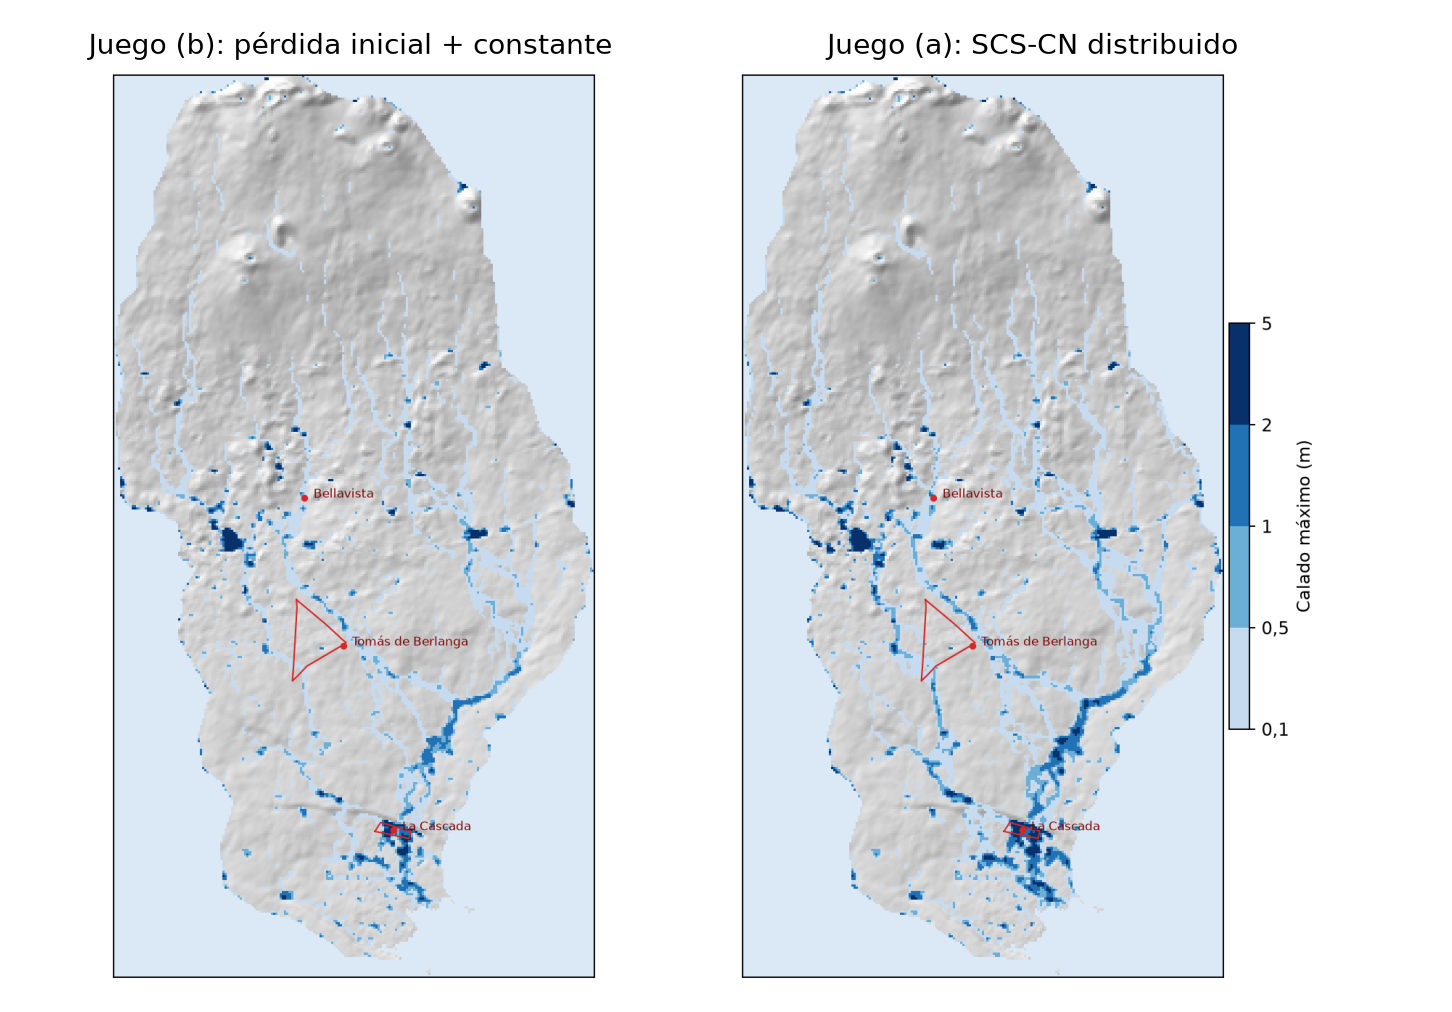
\includegraphics[width=\linewidth]{calado_max_ab.png}
  \caption{Calado máximo simulado desde las 12:00 del 30-oct en la cuenca de Puerto Ayora (malla de 30~m). Izquierda: juego (b), pérdida inicial y constante, el principal. Derecha: juego (a), SCS-CN, como envolvente superior. Escala de 0,1 a 5~m; en rojo, La Cascada, Tomás de Berlanga y Bellavista. Modelo sobre DSM con techos y vegetación, sin calibrar con caudales. Composición de las figuras del script 24 hecha con \texttt{figuras.py}.}
  \label{fig:calado}
\end{figure}

\begin{figure}[tp]
  \centering
  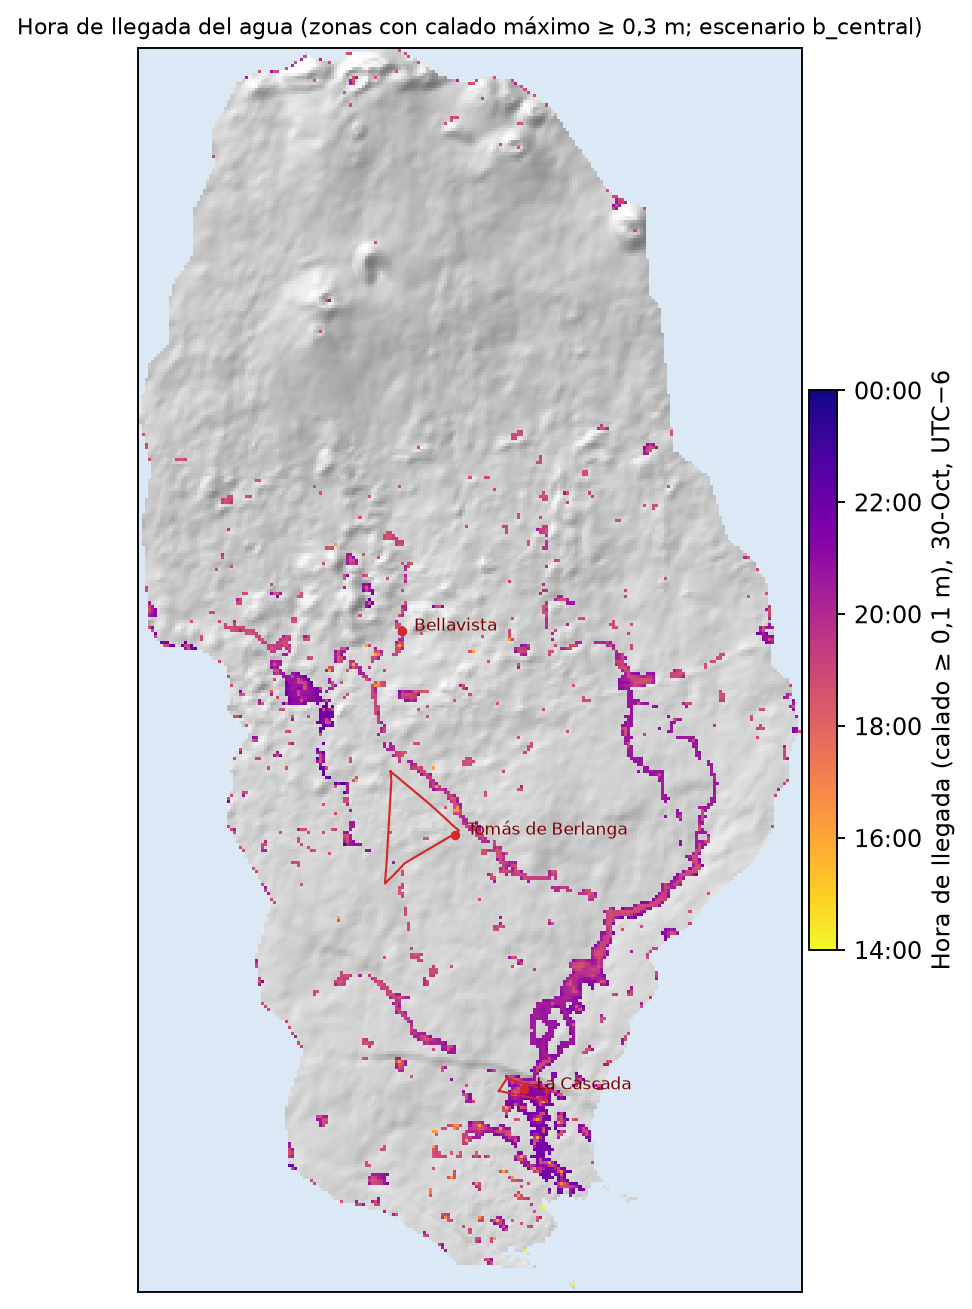
\includegraphics[height=0.42\textheight]{m2d_hora_llegada_b_central.png}
  \caption{Hora de llegada del agua (calado $\geq 0,1$~m) el 30-oct, juego (b). Hora de Galápagos (UTC$-6$).}
  \label{fig:llegada}
\end{figure}

\textbf{Contraste con lo observado.} El testimonio de agua \enquote{hasta dos metros} (prensa, por validar) es compatible con los 1,8--2,4~m del centro y con los 4--4,6~m de la celda más baja, pero no discrimina entre juegos: no se sabe dónde se observó y el DSM tiene ${\pm}2$~m de error. La hora coincide con la \enquote{tarde y noche del 30} de la SNGR. Con el juego (a), el volumen que entra al barrio (3,2~hm³) es el 69\,\% de la escorrentía agregada de su cuenca (4,6~hm³), y el pico (345~m³/s) cae dentro del rango agregado del Informe 2026-04 (325--497~m³/s); el resto queda retenido en depresiones del DSM aguas arriba o sigue escurriendo a las 08:00.

\textbf{Balance de agua del juego (b).} De los 8,18~hm³ de lluvia que superan la pérdida inicial en el dominio, la pérdida constante retira 5,89~hm³ (72\,\%), salen al mar 1,32~hm³ y quedan 0,97~hm³ en tierra al final. Con el juego (a), la lluvia neta es de 5,56~hm³ y salen al mar 3,95~hm³.

\textbf{Contraste con ANUGA.} Los dos motores coinciden en lo esencial (tabla~\ref{tab:anuga}). Los calados puntuales difieren hasta en 0,8~m porque cada malla promedia la cota del DSM de forma distinta en la celda o en el triángulo. El caudal de entrada también difiere (67 frente a 147~m³/s): ANUGA arranca seco a las 17:00 y la sección de control se calcula de otra manera.

\begin{table}[ht]
  \centering\small
  \caption{Contraste entre el esquema de inercia local y ANUGA (juego b, lluvia central).}
  \label{tab:anuga}
  \begin{tabular}{lcc}
    \toprule
    Magnitud & Inercia local (30~m) & ANUGA (20\,400 triángulos) \\
    \midrule
    Nivel máximo en La Cascada & 14,8~m* & 14,5~m* \\
    Hora del máximo & 22:24 & 22:17 \\
    Nivel máximo en Matazarnos & 14,0~m* & 13,9~m* \\
    Superficie con más de 1~m de agua & 89~ha & 89~ha \\
    Calado máximo en el centro de La Cascada & 1,84~m & 2,61~m \\
    Caudal pico de entrada a La Cascada & 147~m³/s & 67~m³/s \\
    Tiempo de cálculo & 55~s & 2,4~h \\
    \bottomrule
  \end{tabular}
\end{table}

\subsection{Validación condicional: el 3--4 de octubre}
El 3 y el 4 de octubre cayeron 112~mm en Los Guayabillos con un máximo de 12,6~mm/h, y no consta inundación en La Cascada. El juego (a) inundaría el barrio esos días; el (b), no (tabla~\ref{tab:validacion}, figura~\ref{fig:validacion}). El 23-oct se descarta para La Cascada porque la lluvia cayó al oeste, fuera de la cuenca; ningún juego lleva agua al barrio ese día.

\begin{table}[ht]
  \centering\small
  \caption{Validación condicional con el 3--4 de octubre (sin inundación reportada, por confirmar, \issue{52}).}
  \label{tab:validacion}
  \begin{tabular}{lccccc}
    \toprule
    Juego & Centro & \makecell{Celda\\más baja} & \makecell{Caudal\\de entrada} & \makecell{Volumen\\que entra} & ¿Cumple? \\
    \midrule
    (a) SCS-CN & 1,18~m & 3,33~m & 27~m³/s & 1,2~hm³ & No: inundaría \\
    (b) $F = 25$~mm/h & 0,00~m & \makecell{0,52~m\\(lluvia local)} & 0~m³/s & 0 & Sí \\
    \bottomrule
  \end{tabular}
\end{table}

\begin{figure}[t]
  \centering
  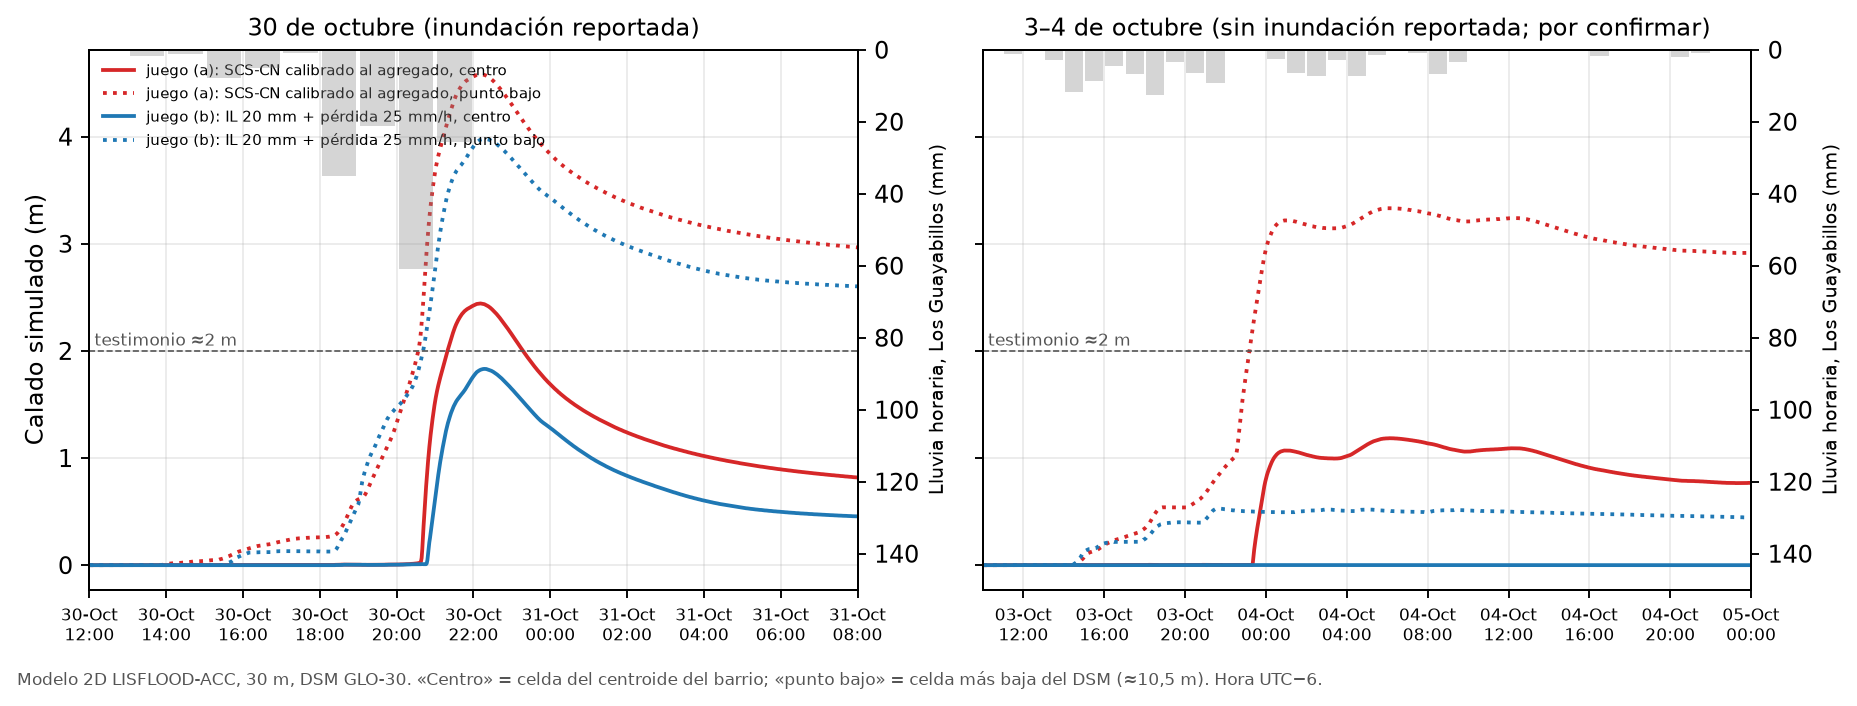
\includegraphics[width=\linewidth]{m2d_validacion.png}
  \caption{Calado simulado en el centro y en la celda más baja de La Cascada con los juegos (a) y (b), con la lluvia horaria de Los Guayabillos. Izquierda: 30-oct (inundación reportada). Derecha: 3--4-oct (sin inundación reportada, por confirmar). La línea discontinua marca el testimonio de ${\approx}\,2$~m.}
  \label{fig:validacion}
\end{figure}

La diferencia está en cómo cada juego reparte las pérdidas. El SCS-CN las reparte según el volumen acumulado: cualquier día de 60--70~mm sobre suelo húmedo produce escorrentía, y un vaso que se llena con decenas de miles de metros cúbicos se inunda. La pérdida constante depende de la intensidad: el 3-oct, con 12,6~mm/h de máximo horario (26~mm/h en 10~min), casi nada supera la capacidad de infiltración del basalto; el 30-oct hubo unas tres horas seguidas a 21--61~mm/h. Aun así, los dos juegos coinciden en que La Cascada se inunda con más de 20--25~mm/h sostenidos durante más de una hora sobre la parte media de la cuenca.

\subsection{Sensibilidad}
\textbf{Pérdida constante.} Cualquier $F \geq 10$~mm/h deja el barrio seco el 3-oct (figura~\ref{fig:barrido}). Con 15--25~mm/h se obtienen 1,8--2,3~m en el centro el 30-oct. El calado varía poco (1,3--2,4~m en todo el barrido), pero \textbf{el caudal pico de entrada varía unas siete veces}, de 47 a 319~m³/s. La validación condicional acota $F$ por abajo, pero no lo fija.

\begin{figure}[t]
  \centering
  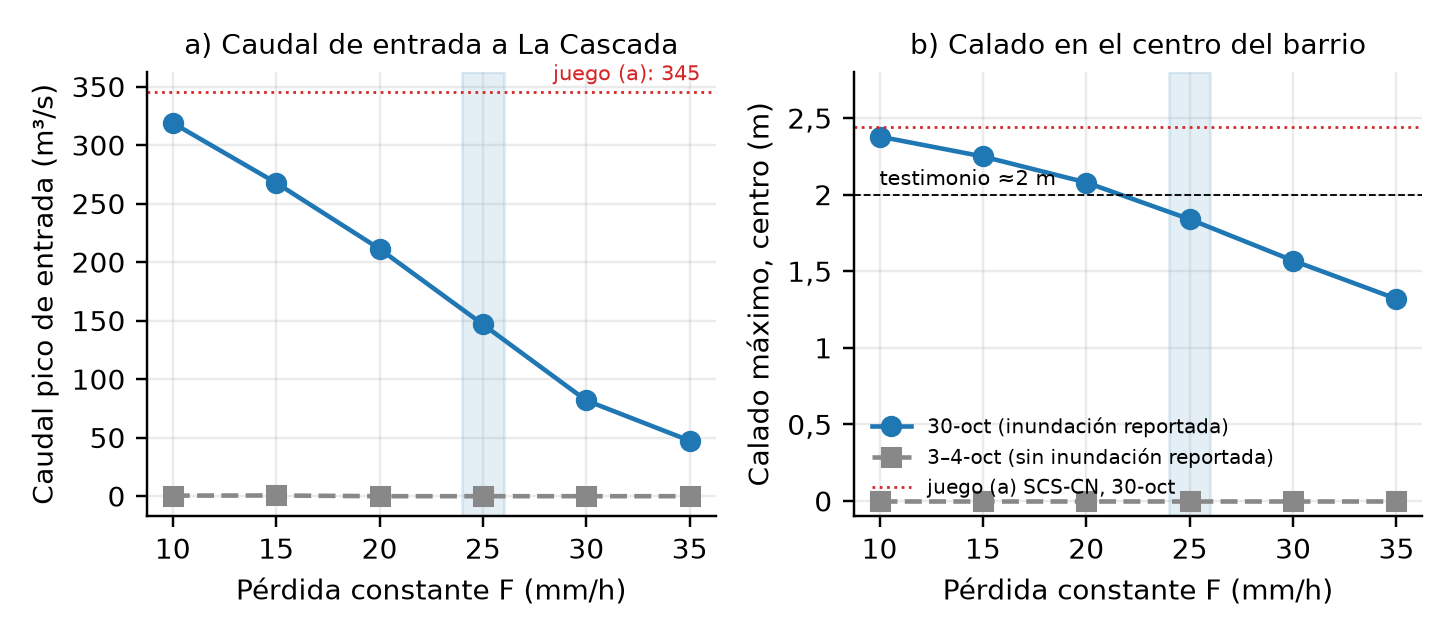
\includegraphics[width=0.95\linewidth]{barrido_f.png}
  \caption{Barrido de la pérdida constante $F$ del juego (b), con $I_L = 20$~mm y la lluvia central. (a) Caudal pico de entrada a La Cascada. (b) Calado máximo en el centro del barrio. Círculos: 30-oct; cuadrados: 3--4-oct. Línea roja punteada: juego (a). Banda azul: valor adoptado (25~mm/h). Figura nueva, generada con \texttt{figuras.py} a partir de los \texttt{resumen\_*.json} del modelo.}
  \label{fig:barrido}
\end{figure}

\begin{table}[ht]
  \centering\small
  \caption{Sensibilidad del modelo 2D (30-oct): calado máximo en el centro de La Cascada y caudal pico de entrada (hora UTC$-6$ entre paréntesis cuando cambia).}
  \label{tab:sensibilidad}
  \begin{tabular}{lcc}
    \toprule
    Variante & Juego (a): centro / entrada & Juego (b): centro / entrada \\
    \midrule
    Central & 2,4~m / 345~m³/s & 1,8~m / 147~m³/s \\
    Lluvia baja ($\times 0,85$; 152~mm) & 2,2~m / 246~m³/s & 1,4~m / 58~m³/s \\
    Lluvia alta (gradiente; ${\approx}\,208$~mm) & 2,7~m / 454~m³/s & 2,0~m / 204~m³/s \\
    Manning $\times 0,6$ & 2,2~m / 413~m³/s (21:34) & 1,8~m / 216~m³/s (21:43) \\
    Manning $\times 1,4$ & 2,6~m / 290~m³/s (22:27) & 1,8~m / 101~m³/s (22:50) \\
    CN 68 en lugar de 76 & 2,2~m / 265~m³/s & --- \\
    \bottomrule
  \end{tabular}
\end{table}

\textbf{Rugosidad, lluvia y CN.} El calado en el barrio va de 1,4 a 2,7~m en todas las variantes de la tabla~\ref{tab:sensibilidad}: lo controlan la cota del umbral de salida y el remanso en Matazarnos y el frente urbano, no el caudal. La rugosidad casi no cambia el calado, pero desplaza el pico unos 30--40~min y cambia el caudal en un factor de 1,4--2. Lo que más pesa en los caudales y en la extensión inundada es el juego de pérdidas.

\textbf{Nivel del mar.} El modelo fija el mar en $+0,75$~m. Según el mareógrafo de Puerto Ayora (IOC, operado por el INOCAR), a la hora del pico el mar estaba entre $+0,13$ y $+0,05$~m y bajando, 0,6--0,7~m por debajo del supuesto [M]; la comparación supone que el cero del DSM coincide con el nivel medio del mareógrafo, algo no comprobado. Con $+0,75$~m quedan bajo el mar desde el inicio 7 celdas de tierra (${\approx}\,0,6$~ha) en la orilla. La Cascada, Matazarnos y el cruce de la Av. Charles Darwin están a 10--15~m* y los controla su propio umbral: el supuesto es conservador para la orilla y neutro para el barrio.

\subsection{San Cristóbal: tormenta trasladada}
Con la tormenta de Los Guayabillos trasladada, la Galápagos concentra el mayor caudal y su desembocadura en Barrio Frío es el punto más expuesto (tabla~\ref{tab:sancristobal}, figura~\ref{fig:sancristobal}). Con la malla de 15~m supera 5~m³/s a las 18:40 y alcanza un calado de 0,3~m a las 20:35, dentro de la hora de máxima lluvia: el margen real desde la lluvia intensa es \textbf{menor de 1~h}. El limitador de Froude frena el flujo en las laderas, así que las horas de llegada están sesgadas hacia tarde. El Progreso es lo primero que se encharca, en depresiones sin salida (0,3~m junto a la escuela desde las 18:30). Como la serie trasladada se corta a las 21:25, los picos coinciden con el final del registro y se leen como mínimos.

\begin{table}[ht]
  \centering\small
  \caption{San Cristóbal: caudal pico por sección (m³/s) en los cuatro escenarios, y edificios con calado máximo $\geq 0,3$~m en la celda de su centroide. Lluvia uniforme; (ii)--(iv) es la tormenta de Santa Cruz trasladada.}
  \label{tab:sancristobal}
  \begin{tabularx}{\linewidth}{>{\raggedright\arraybackslash}Xcccc}
    \toprule
    & \makecell{(i) 100~mm\\SCS tipo II} & \makecell{(ii) Trasladada\\AMC II, 30~m} & \makecell{(iii) Trasladada\\AMC III, 30~m} & \makecell{(iv) Trasladada\\AMC II, 15~m} \\
    \midrule
    Galápagos, desembocadura (Barrio Frío) & 18 & 95 & 127 & 100 \\
    Galápagos, entrada a la ciudad & 4 & 23 & 28 & 19 \\
    Divino Niño, salida & 7 & 16 & 23 & 18 \\
    Alejandro Alvear, salida & 3 & 10 & 15 & 10 \\
    Quebrada del campus, rellano & 0,2 & 2,4 & 3,5 & 2,3 \\
    El Progreso, quebrada IGM & 0,6 & 15 & 17 & 15 \\
    \midrule
    Edificios $\geq 0,3$~m, Puerto Baquerizo (2\,988) & 46 & 187 & 231 & 181 \\
    Edificios $\geq 0,3$~m, El Progreso (206) & 17 & 29 & 30 & 25 \\
    \bottomrule
  \end{tabularx}
\end{table}

\begin{figure}[t]
  \centering
  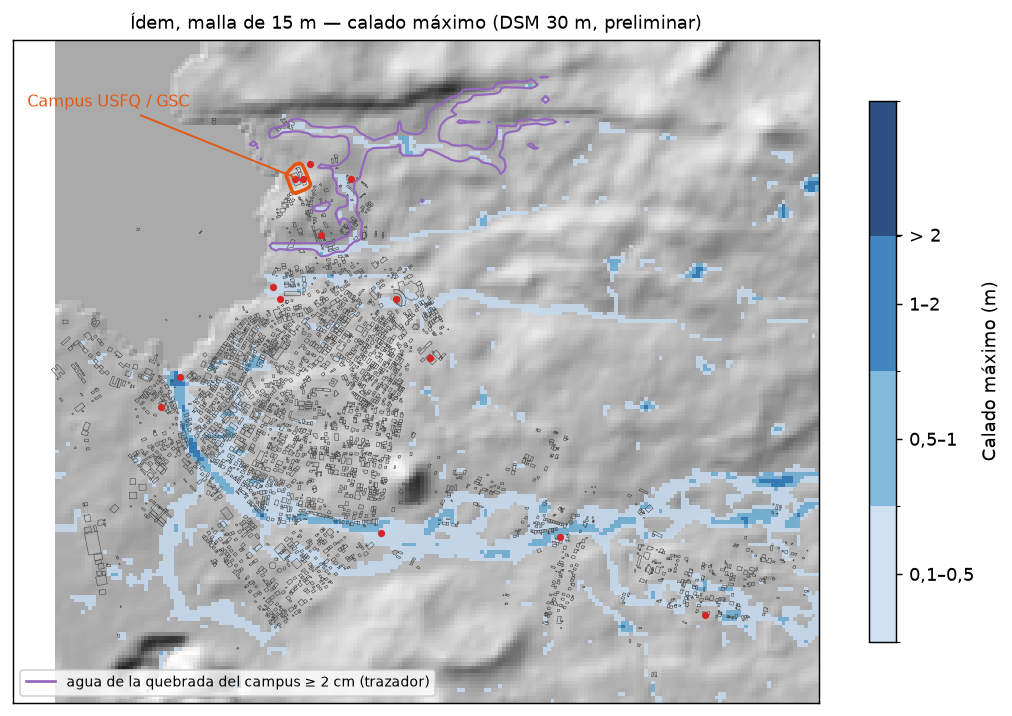
\includegraphics[width=0.82\linewidth]{f_modelo2d_guayabillos_15m_ciudad.png}
  \caption{Calado máximo en Puerto Baquerizo Moreno con la tormenta de Los Guayabillos (Santa Cruz) trasladada, malla de 15~m. En morado, zona donde el agua de la quebrada del campus supera los 2~cm (trazador). No es la lluvia de San Cristóbal (\issue{74}).}
  \label{fig:sancristobal}
\end{figure}

\textbf{Trazadores.} El 67\,\% del agua marcada en la Galápagos sale al mar por la playa de Barrio Frío, y el 75\,\% de la de Divino Niño por Playa de Oro; solo el 1,7\,\% de esta última pasa a la Galápagos. El modelo, por tanto, no reproduce que Divino Niño \enquote{se separe} hacia la Galápagos, como describe el Plan de Acción de la UGR del GAD; no verlo no descarta esa conexión, que depende de calles y obras que una malla de 15--30~m no resuelve. En el campus USFQ\,/\,GSC, un 5--10\,\% del agua de la quebrada cruza el campus como desborde somero, con 0,18--0,47~m³/s y una lámina total de 4--5~cm. Con 100~mm el resultado no es concluyente.

\textbf{Resolución y comparación con el método agregado.} Pasar de 30 a 15~m cambia los caudales en ${\pm}20$\,\% y los calados puntuales hasta en un factor de 2--3 en El Progreso, sin cambiar las conclusiones cualitativas. Con 100~mm, el pico de Barrio Frío (18~m³/s) se parece al SCS agregado (19~m³/s), pero no es una validación: en las cuencas altas el 2D llena primero las microdepresiones del DSM y subestima los caudales con poca lluvia.

% =====================================================================
\section{Discusión y limitaciones}

El modelo cumple lo que se le pidió: reproduce la hora y el orden de magnitud del calado del 30-oct con lluvia medida, y separa ese día de los de octubre sin inundación reportada. Lo hace con un juego de pérdidas que depende de la intensidad, lo que es físicamente coherente con un sustrato de basalto fracturado y cauces efímeros. Pero el ajuste se apoya en un solo evento con inundación y en una validación \emph{condicional}, y el parámetro que la validación acota, la pérdida constante, es justamente el que más cambia el caudal.

\begin{itemize}
  \item \textbf{Calibración.} Un solo evento, sin caudales ni marcas de agua. La validación con el 3--4-oct depende de que esos días realmente no hubo inundación (\issue{52}). $F$ solo está acotado por abajo (${\geq}\,10$~mm/h). El caudal de entrada va de 47 a 319~m³/s con $F$ entre 35 y 10~mm/h: \textbf{no sirve para diseño}.
  \item \textbf{Lluvia.} Puntual y mínima: dos estaciones útiles, ambas fuera de la cuenca, cortadas a las 21:25. La entrada de lluvia se corta a esa hora. El pluviómetro INAMHI M0191 de Puerto Ayora midió unos 135~mm más entre las 22:00 y las 03:00 [M]; si esa lluvia cayó también en la parte media de la cuenca, lo que no se sabe, el vaso siguió recibiendo agua después del máximo que da el modelo.
  \item \textbf{Terreno.} El DSM de 30~m incluye techos y árboles, no representa calles, muros, alcantarillas ni cauces estrechos, y crea depresiones falsas. Los calados absolutos tienen una incertidumbre del orden de ${\pm}1$--2~m.
  \item \textbf{Sin red pluvial.} No hay sumideros, colectores ni pasos bajo vías. En el centro urbano el modelo sobrestima el encharcamiento si los sumideros funcionan y lo subestima si se obstruyen.
  \item \textbf{Mar a nivel fijo} en Santa Cruz ($+0,75$~m) y salida libre en San Cristóbal. Desde septiembre el mar está 0,26--0,51~m por encima de su marea astronómica en Puerto Ayora y Baltra [M]: una tormenta así con pleamar de sicigia daría ${\approx}\,1,3$~m más de mar en el último tramo de la salida, sin contar el oleaje (\issue{13}).
  \item \textbf{San Cristóbal} corre con la lluvia de otra isla, sin calibración alguna y con $\theta = 1$ y limitador de Froude. La lluvia medida por el USFQ GSC el 31-oct en la parte alta (91--150~mm en el día [M]) está pendiente de simular (\issue{74}).
\end{itemize}

% =====================================================================
\section{Conclusiones y trabajo futuro}
\begin{enumerate}
  \item El esquema de inercia local con $\theta = 0,8$ reproduce en menos de un minuto por evento la secuencia del 30-oct en La Cascada: llegada al centro a las 20:40--20:55 y máximo a las 22:10--22:25, con 1,8--2,4~m de calado.
  \item Solo el juego de pérdida inicial y constante (b) cumple a la vez con el 30-oct y con el 3--4-oct; se adopta como principal y el SCS-CN (a) queda como envolvente superior.
  \item ANUGA confirma el nivel máximo (14,5 frente a 14,8~m) y la superficie con más de 1~m (89~ha), pero no el caudal de entrada.
  \item El calado en el barrio es robusto (1,3--2,7~m en todas las variantes); el caudal no (47--454~m³/s). El modelo explica el mecanismo, pero no sirve para dimensionar obras sin aforos.
  \item En San Cristóbal, con lluvia trasladada, Barrio Frío desborda dentro de la hora de máxima lluvia y El Progreso se encharca primero.
\end{enumerate}

Para avanzar hacen falta:
\begin{itemize}
  \item confirmar si hubo inundación el 3-oct, el 23-oct y el 1--2-nov (\issue{52}) y un registro de inundaciones con hora y profundidad (\issue{80});
  \item marcas de agua con GNSS (\issue{2}) y aforos o huellas de crecida (\issue{9}) para calibrar $F$;
  \item incorporar la lluvia del INAMHI M0191 (\issue{3}) y correr San Cristóbal con su lluvia medida (\issue{74});
  \item un modelo del terreno de dron o LiDAR (\issue{16}) antes de bajar a 10--15~m, y la red de drenaje urbano (\issue{5}, \issue{27});
  \item el nivel del mar observado como condición de borde (\issue{13}).
\end{itemize}

\section*{Disponibilidad de datos y código}
{\small\sloppy Todo el cálculo es reproducible desde el repositorio público \emph{mayait/sosgalapagos-datos}, en la carpeta \texttt{geodatos/}:
\begin{itemize}
  \item \texttt{scripts/24\_modelo2d\_santa\_cruz.py}: motor de inercia local y contraste con ANUGA (\texttt{--motor lisflood|anuga}), escenarios, barrido de $F$ (\texttt{F\_PERM}) y figuras;
  \item \texttt{scripts/25\_modelo2d\_san\_cristobal.py}: motor de San Cristóbal (numba), escenarios y trazadores.
\end{itemize}
Salidas y textos de método:
\begin{itemize}
  \item \texttt{geodatos/estudios/santa-cruz/datos/modelo2d/<escenario>/}: \texttt{resumen\_*.json}, \texttt{series\_puntos.csv}, \texttt{caudales\_secciones.csv} y \texttt{calado\_max\_clases.geojson};
  \item \texttt{geodatos/estudios/san-cristobal/datos/modelo2d/}: \texttt{resumen\_modelo2d.json} y series por escenario;
  \item \texttt{geodatos/estudios/santa-cruz/texto/09\_modelo2d.md};
  \item \texttt{geodatos/estudios/san-cristobal/texto/12\_modelo2d.md}.
\end{itemize} La figura~\ref{fig:barrido} se genera con \texttt{informes/2026-06-modelo-2d/figuras.py}. Este informe se compila con \texttt{informes/compilar.sh 2026-06-modelo-2d}.\par}

\bibliographystyle{sosg}
\bibliography{referencias,bib-2026-06}

\end{document}
